
\begin{keynote}
    {Human defensive reactions and their role in approach-avoidance decision making}
    {Karin Roelofs}
    {Thursday 09:15 - 10:15 | ORT}
    {Donders Institute for Brain Cognition and Behavior, Radboud University Nijmegen}

    Behavioural scientists often assume that automatic defensive threat reactions, while essential in explaining animal behavior, only have limited value when it comes to understanding human behavior. There is, however, increasing evidence that defensive reactions, such as freezing, have an impact on subsequent approach-avoidance decisions under acute threat in humans. Understanding the mechanisms that drive such decisions is particularly relevant for patients with anxiety disorders, whose persistent avoidance is key to the maintenance of their anxiety. In recent years, computational psychiatry has made substantial progress formalizing the mechanisms through which we make (mal)adaptive decisions. However, most current models simply ignore the transient psychophysiological state of the decision maker. Here, I argue that the balance between para-sympathetic and sympathetic activity is instrumental in driving the psychophysiological state of freezing, and that it influences approach-avoidance decisions under acute threat in different ways. To illustrate, I first explore the effects of freezing on different kinds of human action decisions under threat. Next, I discuss recent translational (rodent-human) work that has helped to characterize the neural mechanisms implicated in animal and human defensive freezing. Finally, through two prospective longitudinal studies, I show that individual differences in susceptibility to freezing are predictive of the development of anxiety symptoms. 
    Overall, this work suggests that defensive threat reactions and associated psychophysiological states not only affect acute decision making, but also predict long-term symptom development. As such, these factors have great importance for resilience research, and should constitute an integral part of any theory of human decision making.

    \vspace*{1cm}

    \begin{figure}[H]
        \raggedleft
        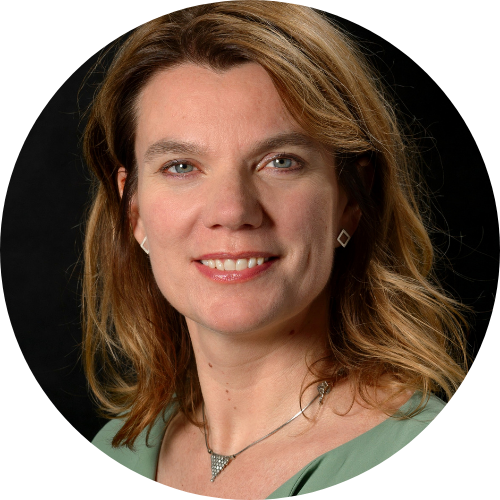
\includegraphics[width=0.24\textwidth]{tex/images/keynote_speaker/roeloefs_cropped.png}
    \end{figure}

\end{keynote}
